\documentclass[
   paper=a4,
   twoside=false,
   parskip=half,
   listof=entryprefix,
   listof=totoc,
   index=totoc,
   bibliography=totoc,
   headsepline,
]{scrbook}

\usepackage{silence}
\WarningFilter{biblatex}{File 'ngerman-iso.lbx'}
\WarningFilter{biblatex}{'\mainlang'}
\WarningFilter{biblatex}{Bibliography string 'online' untranslated}
\WarningFilter{hyperref}{Token not allowed in a PDF string}

%%%%%%%%%%%%%%%%%%%%%%%%%%%%%%%%%%%%%%%%%%%%%%%%%%%%%%%%%%%%%%%%%%%%%%%%%%%%%%
% Fonts Fonts Fonts
%%%%%%%%%%%%%%%%%%%%%%%%%%%%%%%%%%%%%%%%%%%%%%%%%%%%%%%%%%%%%%%%%%%%%%%%%%%%%%
\usepackage[utf8]{inputenc}
\usepackage[ngerman]{babel}
\usepackage[T1]{fontenc}

\usepackage{scrhack}
\usepackage{pdfpages,graphicx,subcaption,lastpage,xspace}
\graphicspath{ {./images} }
\usepackage{float,xcolor,csquotes,microtype,etoolbox}
\MakeOuterQuote{"}
\usepackage[automark,markcase=ignoreuppercase,autooneside=false]{scrlayer-scrpage}
\usepackage[official]{eurosym}
\usepackage[breaklinks,colorlinks,linkcolor=black,citecolor=black,filecolor=black,urlcolor=black]{hyperref}

%%%%%%%%%%%%%%%%%%%%%%%%%%%%%%%%%%%%%%%%%%%%%%%%%%%%%%%%%%%%%%%%%%%%%%%%%%%%%%
% Listings Paket
%%%%%%%%%%%%%%%%%%%%%%%%%%%%%%%%%%%%%%%%%%%%%%%%%%%%%%%%%%%%%%%%%%%%%%%%%%%%%%
\usepackage{listings,caption}
\definecolor{codebg}{rgb}{0.95,0.95,0.95}
\lstset{
   basicstyle =\ttfamily\color{black}\small,
   keywordstyle =,
   commentstyle =\color{teal},
   stringstyle =\itshape,
   tabsize=2,
   breaklines=true,
   captionpos=b,
   breakatwhitespace,
   backgroundcolor={\color{codebg}},
   basewidth=0.5em,
}
\lstloadlanguages{
   bash,
}
\usepackage{pmboxdraw}

%%%%%%%%%%%%%%%%%%%%%%%%%%%%%%%%%%%%%%%%%%%%%%%%%%%%%%%%%%%%%%%%%%%%%%%%%%%%%%
% Bibliography
%%%%%%%%%%%%%%%%%%%%%%%%%%%%%%%%%%%%%%%%%%%%%%%%%%%%%%%%%%%%%%%%%%%%%%%%%%%%%%
\setuptoc{toc}{totoc}

\usepackage[
   backend=biber,
   urldate=long,
   style=iso-authoryear,
   natbib=true,
   useauthor=true,
   mincitenames=1,
   maxcitenames=3
]{biblatex}
\addbibresource{./bib/online.bib}
\addbibresource{./bib/book.bib}

\DeclareNameAlias{default}{family-given/given-family}

\renewcommand*{\finalnamedelim}{\addspace{}und\space}
\AtEveryCite{
   \renewcommand*{\multinamedelim}{,\space}
   \renewcommand*{\nameyeardelim}{\space}
}

\AtBeginBibliography{
   \renewcommand*{\multinamedelim}{,\space}
}
\AfterTOCHead[lof]{\appto\autodot{:}}

%%%%%%%%%%%%%%%%%%%%%%%%%%%%%%%%%%%%%%%%%%%%%%%%%%%%%%%%%%%%%%%%%%%%%%%%%%%%%%
% Fussnoten
%%%%%%%%%%%%%%%%%%%%%%%%%%%%%%%%%%%%%%%%%%%%%%%%%%%%%%%%%%%%%%%%%%%%%%%%%%%%%%
\deffootnote{1.5em}{1em}{\makebox[1.5em][l]{\thefootnotemark}}
\addtolength{\skip\footins}{\baselineskip}
\setlength{\dimen\footins}{10\baselineskip}
\interfootnotelinepenalty=10000  % Verhindert das Fortsetzen von Fussnoten

%%%%%%%%%%%%%%%%%%%%%%%%%%%%%%%%%%%%%%%%%%%%%%%%%%%%%%%%%%%%%%%%%%%%%%%%%%%%%%
% Commands
%%%%%%%%%%%%%%%%%%%%%%%%%%%%%%%%%%%%%%%%%%%%%%%%%%%%%%%%%%%%%%%%%%%%%%%%%%%%%%
\newcommand{\workDatum}{\today\xspace}
\newcommand{\workDateTime}{\today{} - \thistime\ Uhr}
\newcommand{\workFirma}{<Firma>\xspace}
\newcommand{\workTitel}{<Titel>}
\newcommand{\workNameStudent}{<Student>\xspace}
\newcommand{\workTyp}{<Arbeit>\xspace}

\newcommand{\www}[1]{\href{http://#1}{#1}}
\newcommand{\wwwhttp}[1]{\href{#1}{#1}}
\newcommand{\wwwlink}[1]{\footnote{\www{#1}}}

\newcommand{\zB}{\mbox{z.\,B.}\xspace}
\newcommand{\ua}{\mbox{u.\,a.}\xspace}
\newcommand{\dah}{\mbox{d.\,h.}\xspace}
\newcommand{\uAe}{\mbox{u.\,a.}\xspace}

\newcommand{\refp}[1]{Seite~\pageref{#1}\xspace}
\newcommand{\refk}[1]{Kapitel~\ref{#1}\xspace}
\newcommand{\refa}[1]{Abbildung~\ref{#1}\xspace}
\newcommand{\reft}[1]{Tabelle~\ref{#1}\xspace}
\newcommand{\reflst}[1]{Listing~\ref{#1}\xspace}

\newcommand{\engl}[1]{(engl: \textit{#1})\xspace}

%%%%%%%%%%%%%%%%%%%%%%%%%%%%%%%%%%%%%%%%%%%%%%%%%%%%%%%%%%%%%%%%%%%%%%%%%%%%%%
% Kopf und Fusszeilen
%%%%%%%%%%%%%%%%%%%%%%%%%%%%%%%%%%%%%%%%%%%%%%%%%%%%%%%%%%%%%%%%%%%%%%%%%%%%%%
\usepackage{scrtime}
\pagestyle{scrheadings}
\clearpairofpagestyles
\ihead[]{\leftmark}
\ohead[]{\rightmark}
\counterwithout{footnote}{chapter}
\ifoot[\workDateTime]{\workDateTime}
\ofoot[\pagemark]{\pagemark}

%%%%%%%%%%%%%%%%%%%%%%%%%%%%%%%%%%%%%%%%%%%%%%%%%%%%%%%%%%%%%%%%%%%%%%%%%%%%%%
% Acronyms
%%%%%%%%%%%%%%%%%%%%%%%%%%%%%%%%%%%%%%%%%%%%%%%%%%%%%%%%%%%%%%%%%%%%%%%%%%%%%%
\usepackage{acro}

\DeclareAcronym{html}{short=HTML,long=HyperText Markup Language}
\DeclareAcronym{js}{short=JS,long=JavaScript}

%%%%%%%%%%%%%%%%%%%%%%%%%%%%%%%%%%%%%%%%%%%%%%%%%%%%%%%%%%%%%%%%%%%%%%%%%%%%%%
% Dokument
%%%%%%%%%%%%%%%%%%%%%%%%%%%%%%%%%%%%%%%%%%%%%%%%%%%%%%%%%%%%%%%%%%%%%%%%%%%%%%
\begin{document}

    \newcommand{\HRule}[2]{\noindent\rule[#1]{\linewidth}{#2}}
\newcommand{\vlinespace}[1]{\vspace*{#1\baselineskip}}
\newcommand{\titleemph}[1]{\textbf{#1}}
\begin{titlepage}
    \sffamily
    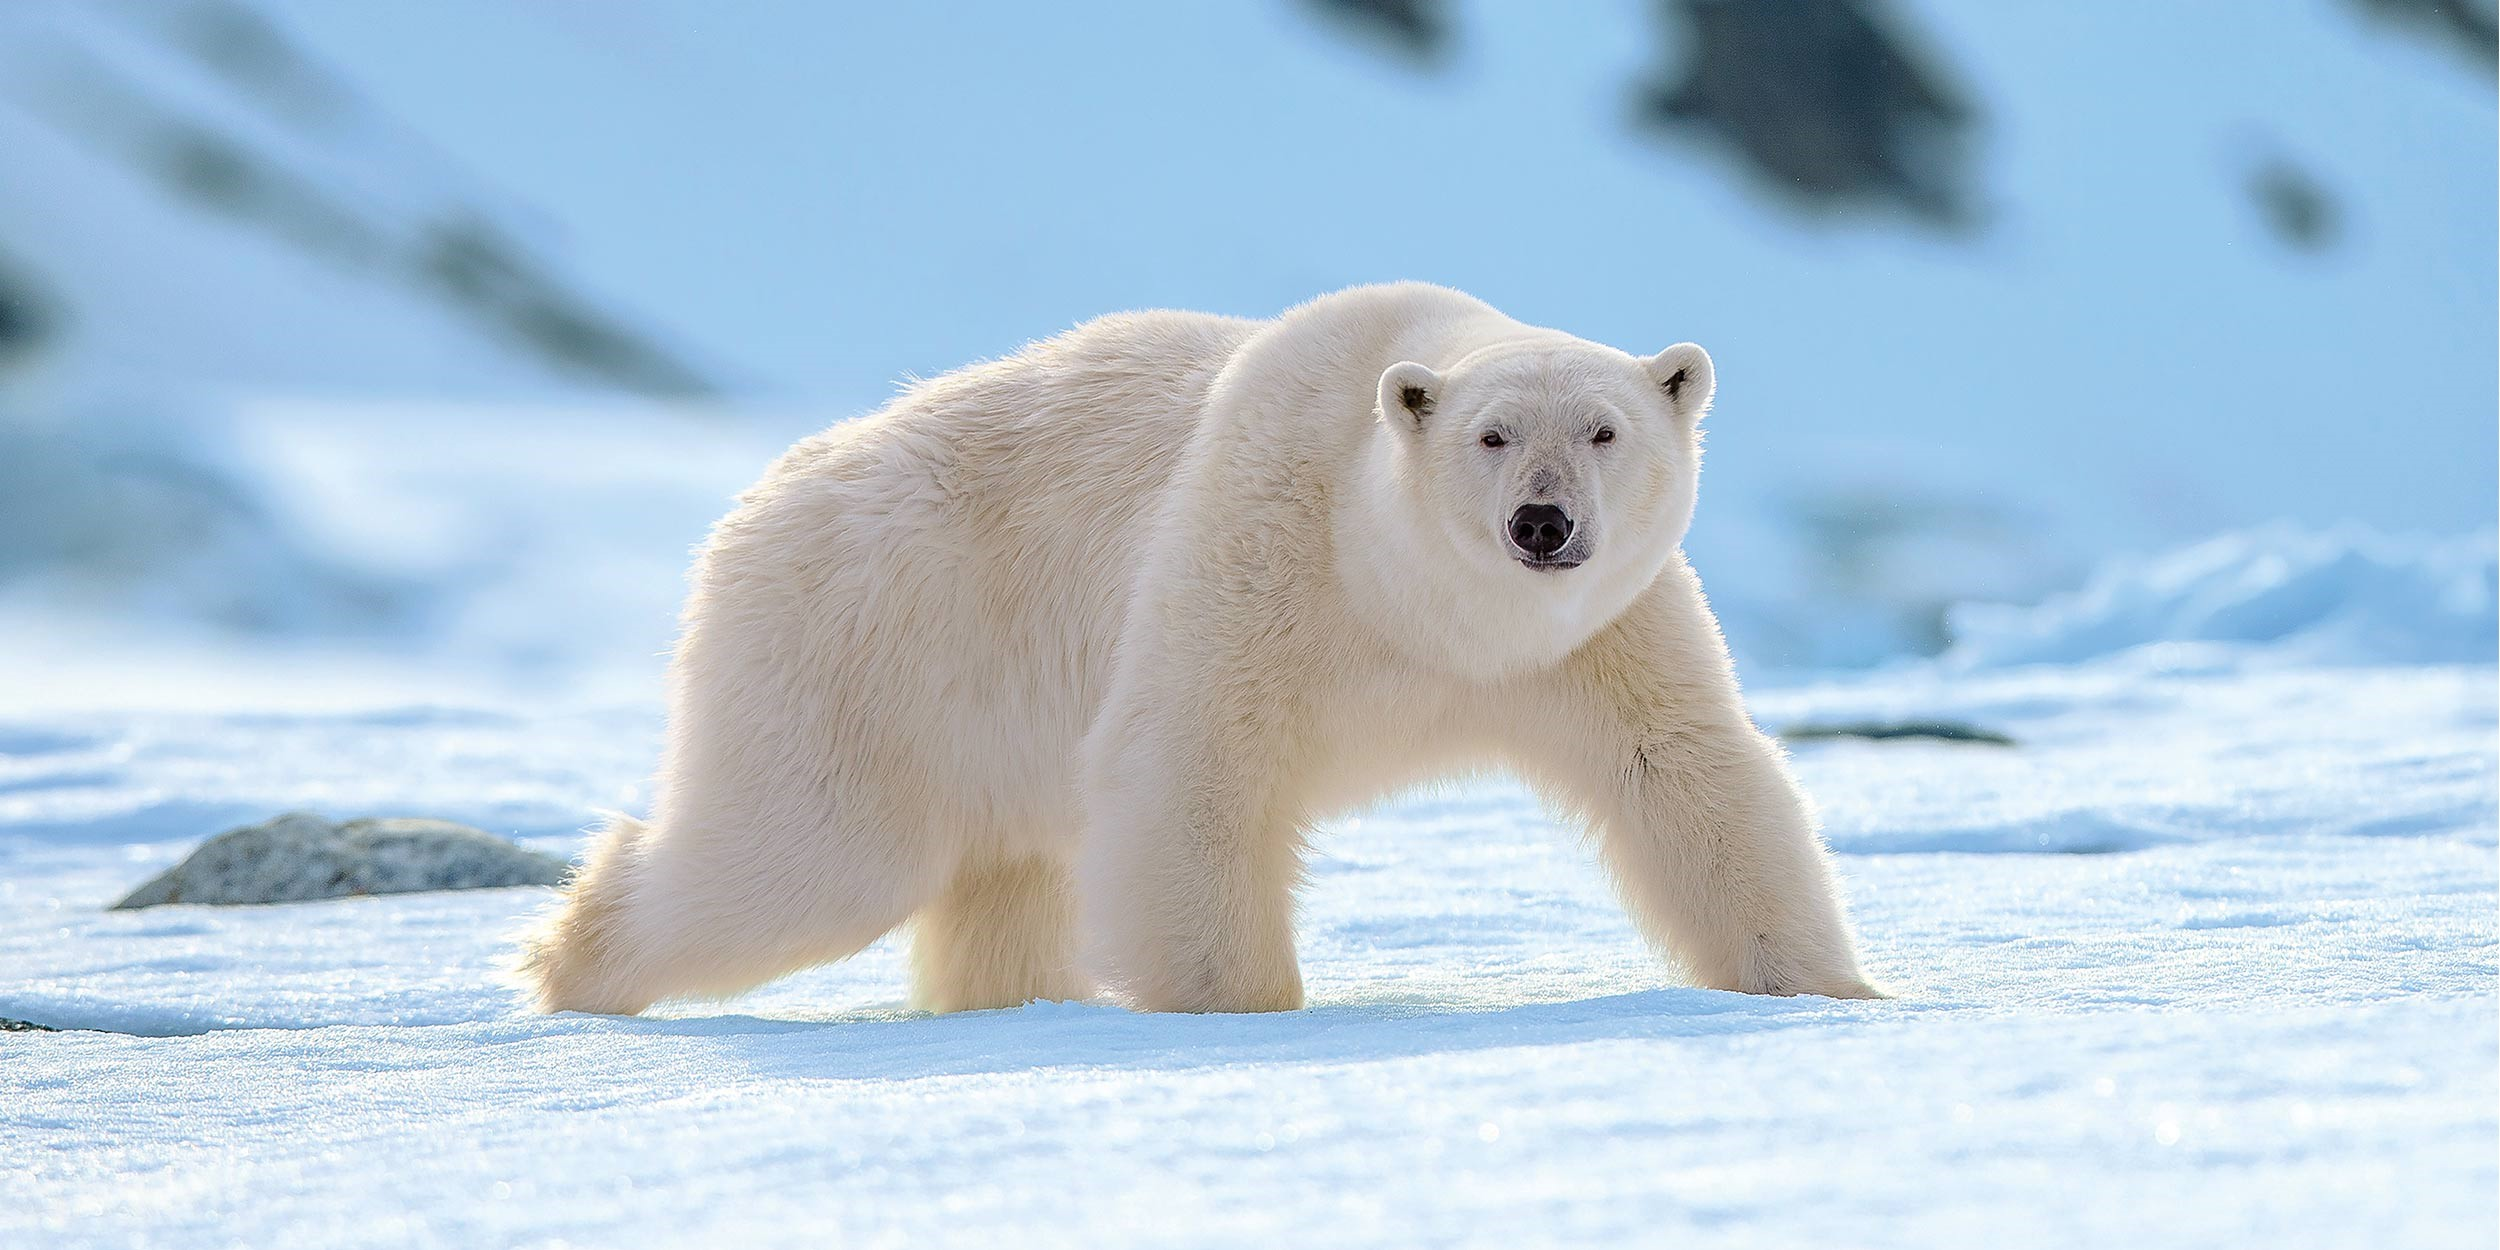
\includegraphics[width=5cm]{example}
    \hfill
    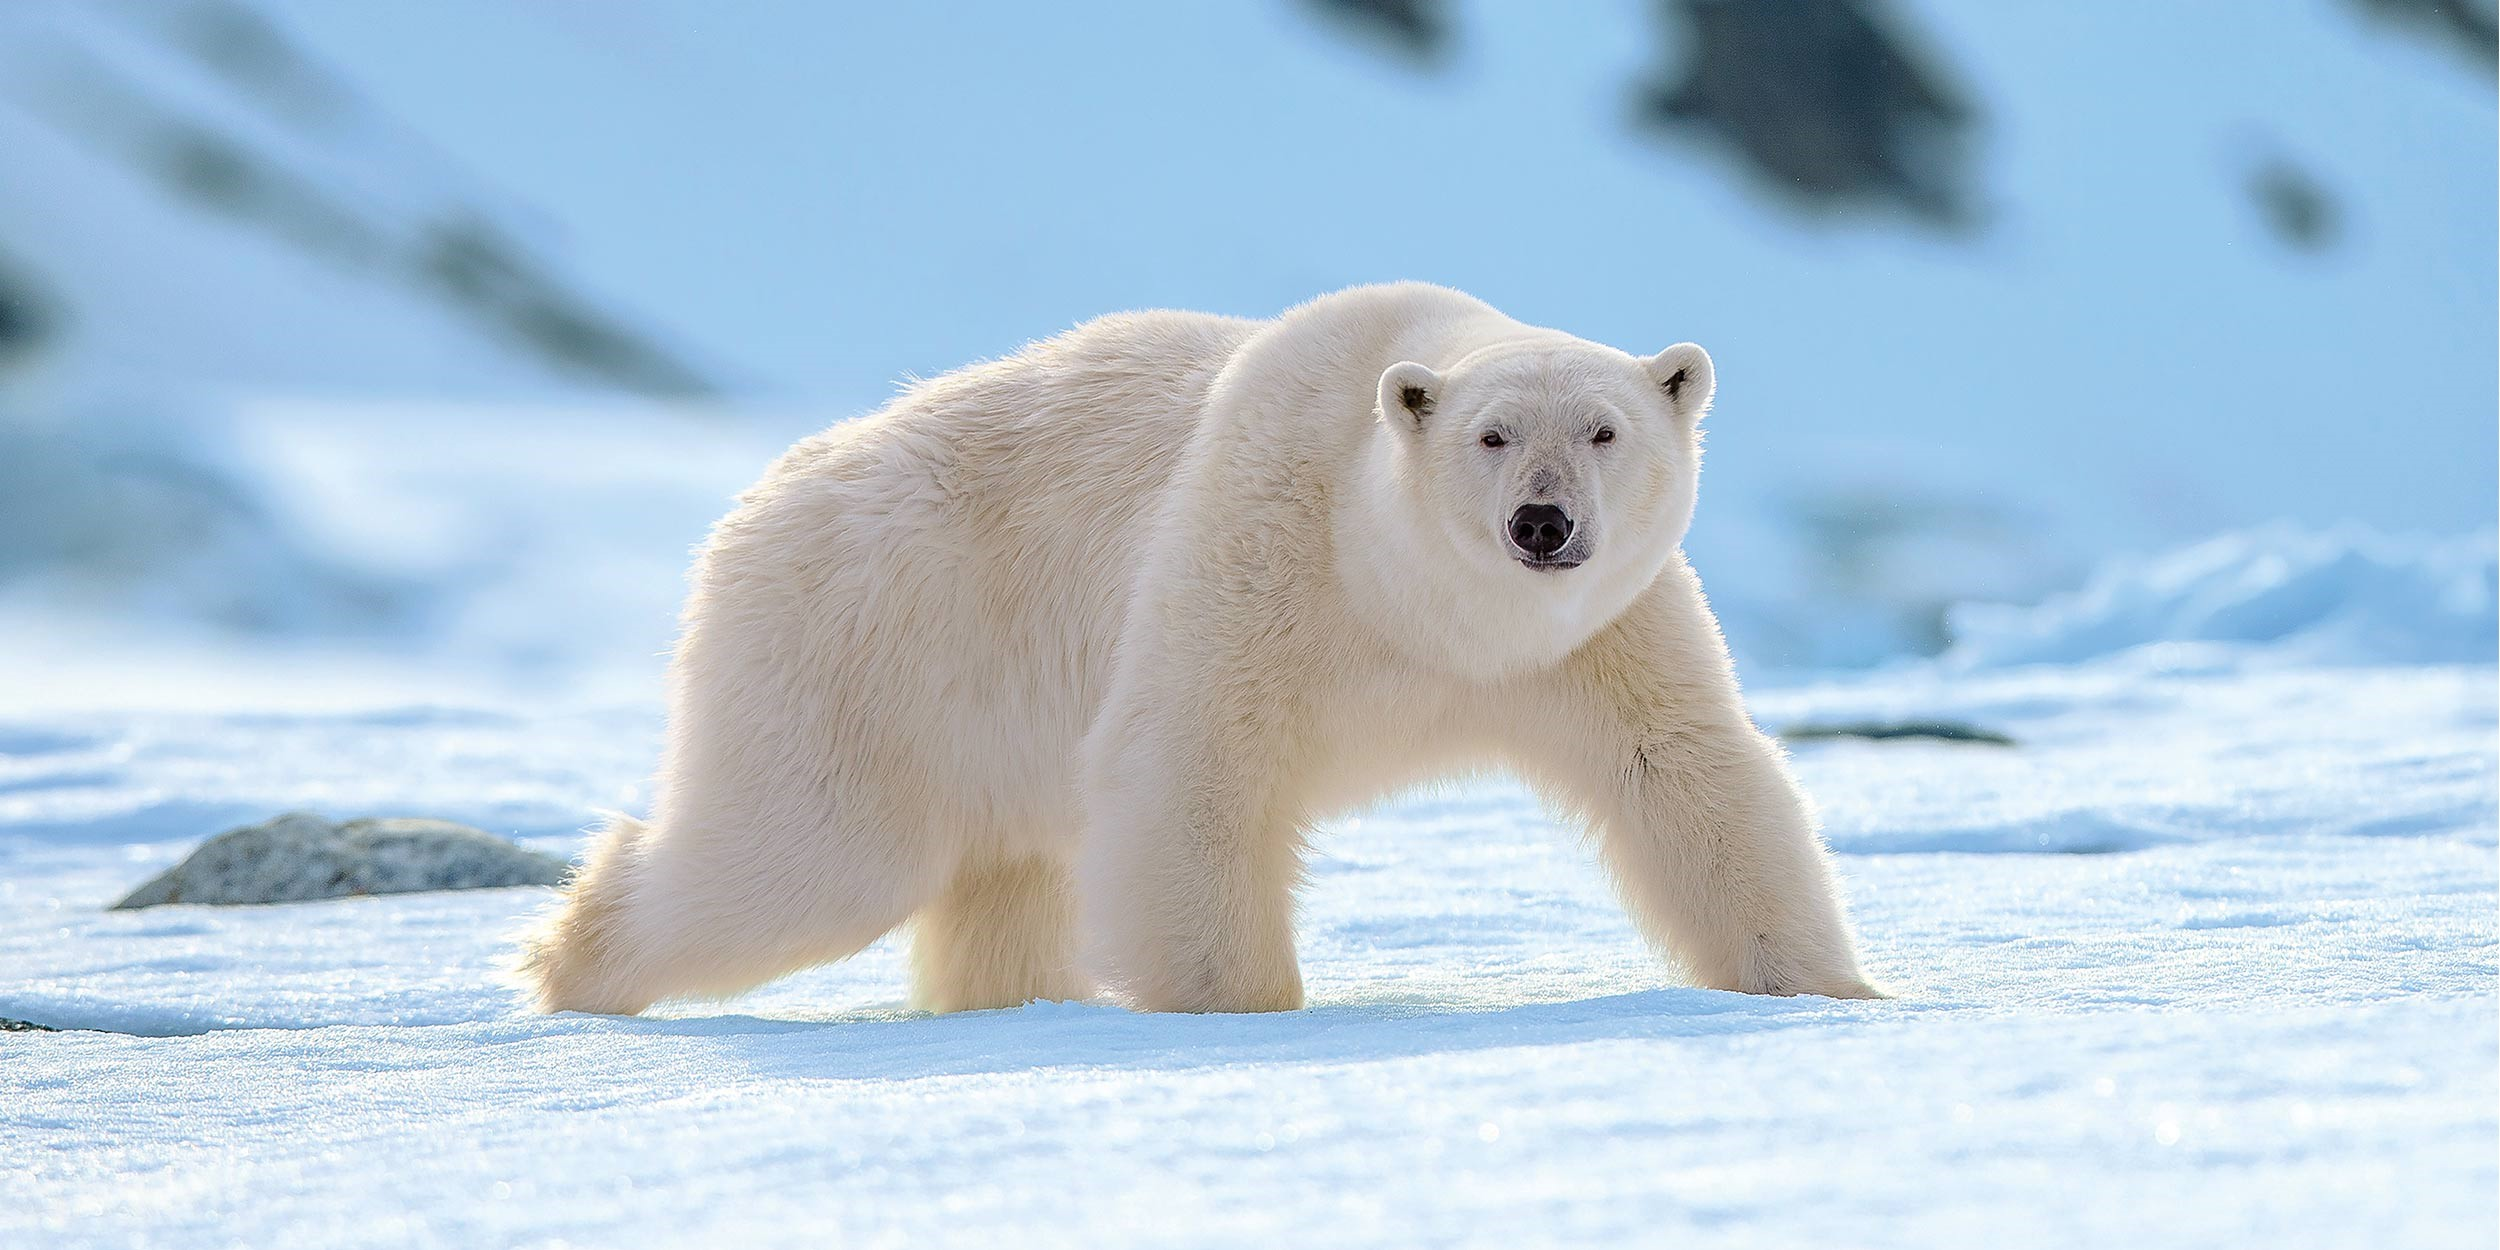
\includegraphics[width=5cm]{example}
    \HRule{13pt}{1pt}
    \centering
    \vlinespace{5}\\
    \workTyp\\
    \begin{Large}
        \textbf{Titel}\\
        \textbf{und mehr}\\
    \end{Large}
    \vlinespace{4}
    im Studiengang\\
    <Studiengang>\\
    am \workDatum\\
    \vlinespace{4}
    vorgelegt von\\
    \begin{Large}
        \textbf{\workNameStudent}\\
    \end{Large}
    \vlinespace{1}
    Matrikelnummer: <12345>
    \vfill
    \raggedright{}
    \HRule{13pt}{1pt} \\
    \titleemph{Erstprüfer:} Prof. <wx>\\
    \titleemph{Zweitprüfer:} Prof. <yz>
\end{titlepage}
    \chapter*{Eidesstattliche Erklärung}

Hiermit versichere ich, die vorliegende Arbeit selbstständig und unter ausschließlicher Verwendung der angegebenen Literatur und Hilfsmittel erstellt zu haben.

Die Arbeit wurde bisher in gleicher oder ähnlicher Form keiner anderen Prüfungsbehörde vorgelegt und auch nicht veröffentlicht.

\begin{tabbing}
          Esslingen, den \workDatum~~\= \rule{5cm}{0.3mm}\\
                                                                                                    \> Unterschrift
\end{tabbing}


    \tableofcontents
    \newpage
    \listoffigures
    \printacronyms
    \addcontentsline{toc}{chapter}{Abkürzungen}

    \section{Example}

\begin{figure}[H]
    \begin{center} 
        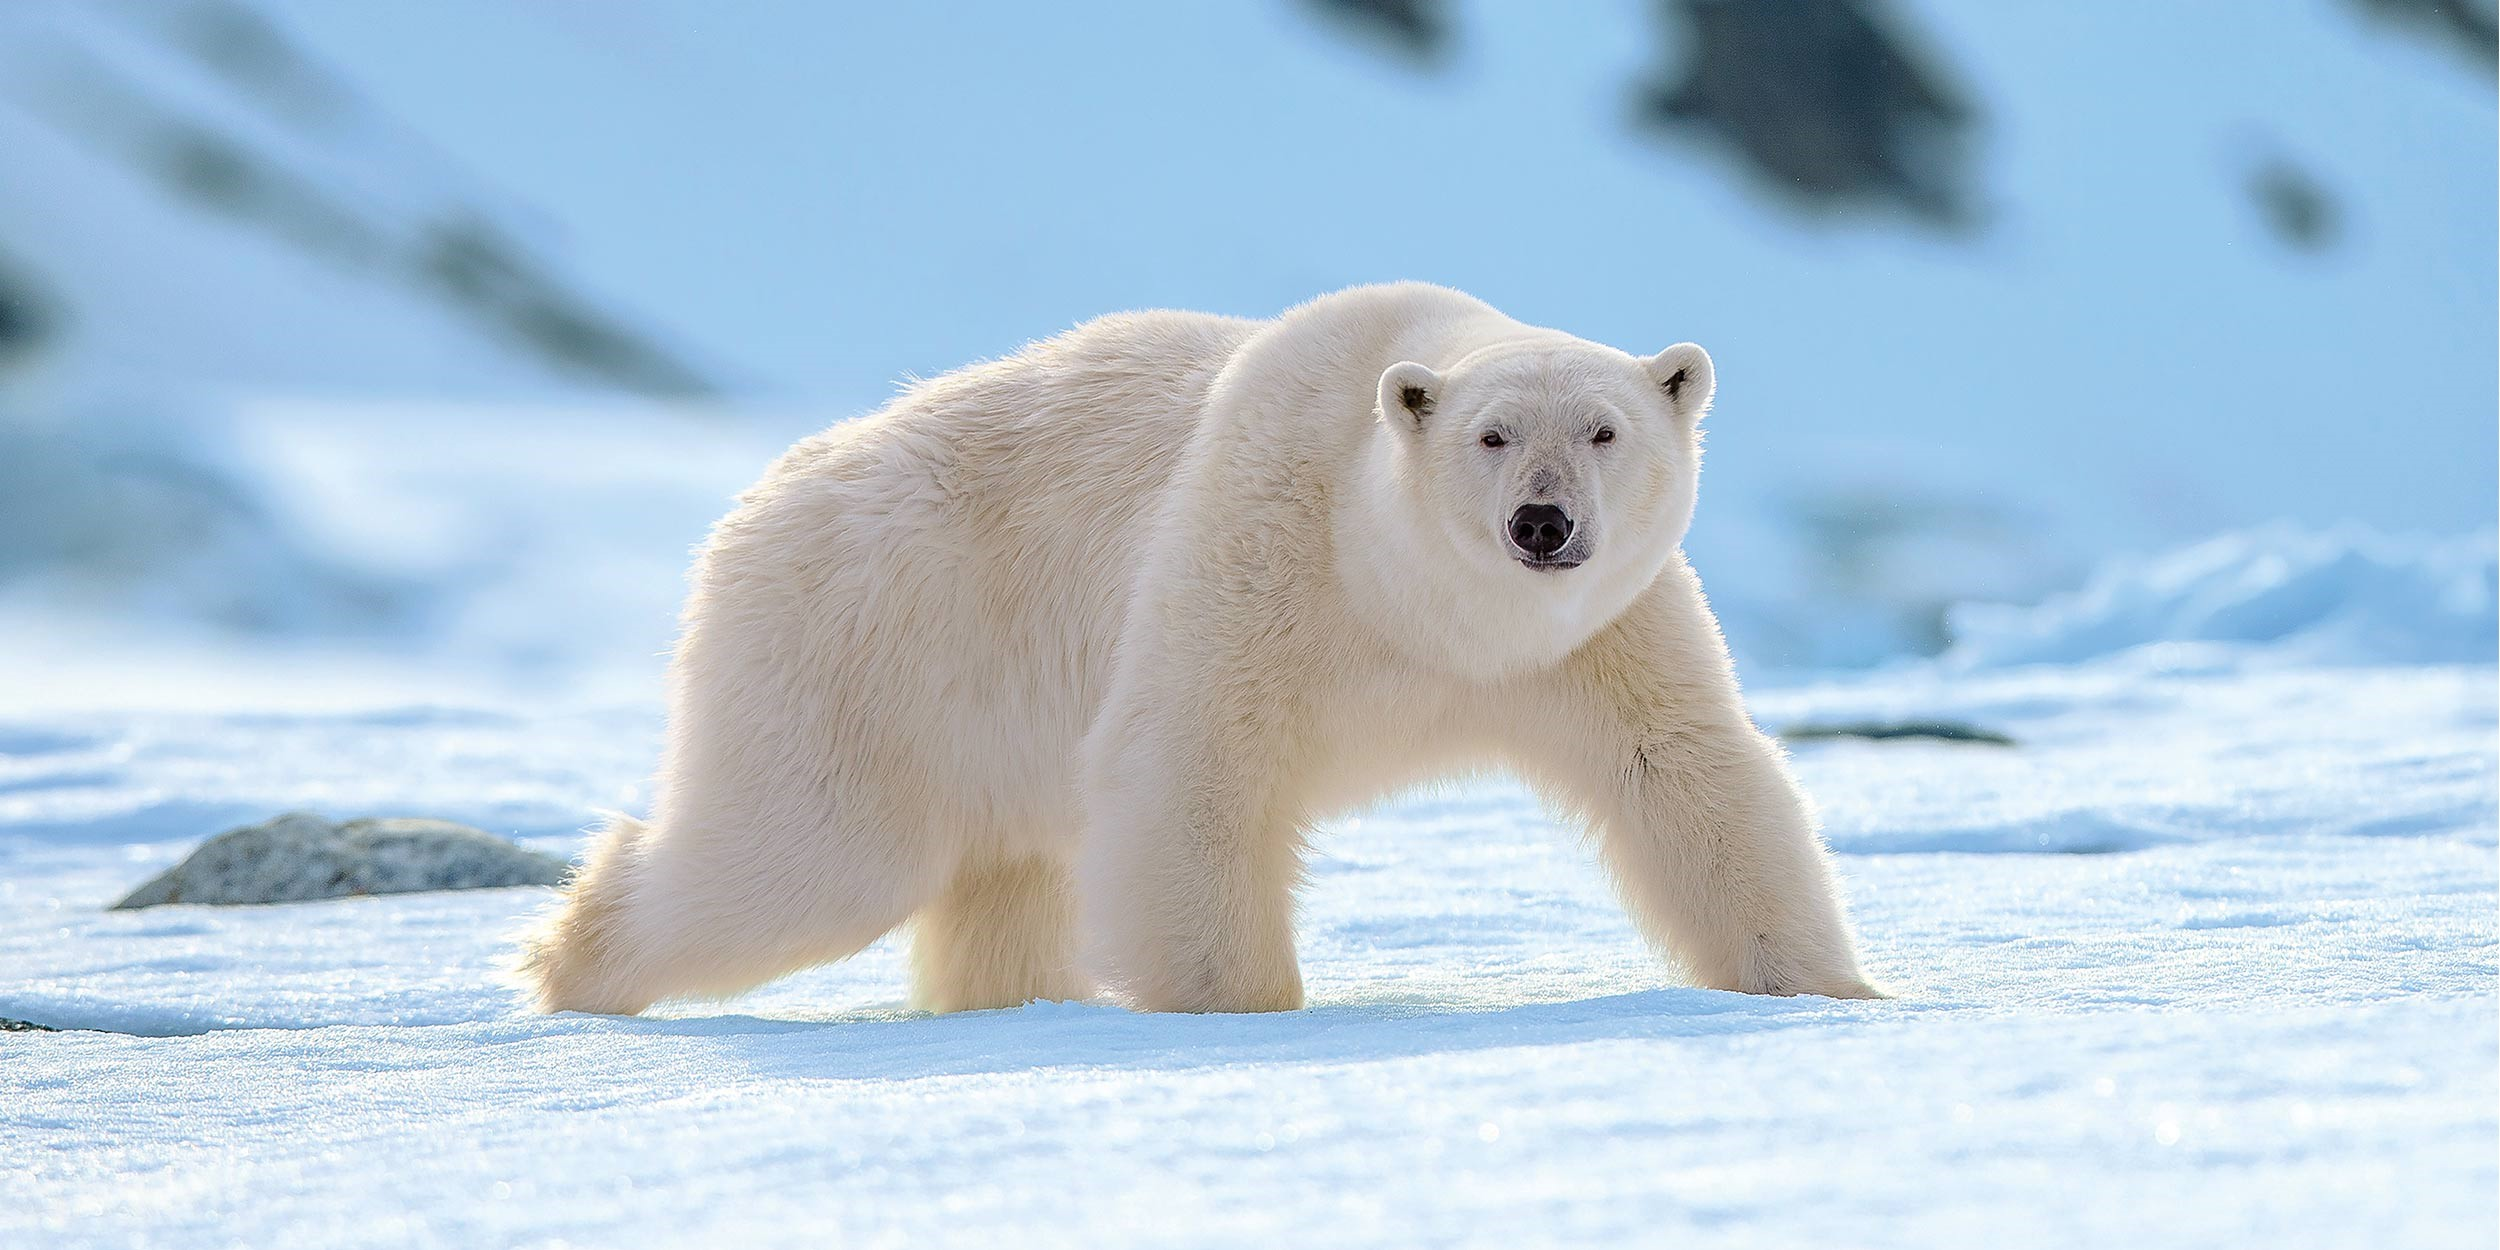
\includegraphics[width=0.8\textwidth]{example}
        \caption{Example Image}
        \label{fig:example}
    \end{center}
\end{figure}

\cite[vgl. dazu][]{example-book}

\cite[vgl. dazu][]{example-online}

\newpage

\begin{lstlisting}[language=Bash]
#!/bin/bash

echo "Hello World"
\end{lstlisting}

\begin{lstlisting}[language=Python]
# same in python

print("Hello World")
\end{lstlisting}

\begin{verbatim}
$ sudo apt-get update
$ sudo apt-get install python
\end{verbatim}


    \printbibliography[title=Literaturverzeichnis]

\end{document}